\section{Signal Expectation}
Our signal expectation is quantified through both an acceptance, composed
of a geometric acceptance and a pre-tagged efficiency, and an 
efficiency of the \btag for the $b$-tagged sample. The following
section describes the signal MC generation with helicity re-weighting,
and the calculations of acceptance and efficiency for the signal.

\subsection{Event Generation}
We have generated the FCNC signal MC samples using the \pyth event
generator, version 6.216~\cite{Sjostrand:2003wg}, for the $1.12\invfb$
run range (runs 141544--222426) and a top mass of $175\gevcsq$. The
FCNC decay \tZq is not in the list of standard decays within
\pyth; therefore, we have redefined the decay products of the $t
\rightarrow W d$ decay channel, which has a negligible branching fraction, 
to be a $Z$ boson and a $c$ or $u$ quark. 

For the main FCNC signal sample, we force one top quark into the SM
decay \tWb and the other top quark to our FCNC decay \tZc
letting \pyth decide randomly whether the
$t$ or $\tbar$ decays to a $W$ and a $b$ quark.  This decay is the
dominant contribution to the FCNC signal acceptance.  We have
generated 0.1 events per $0.5\unit{nb^{-1}}$, yielding a total of
539,445 signal events. The decay of the $Z$ is forced into \ee or
\mm pairs, and the decay of the $W$ is forced into \Wqq.

In addition to the main FCNC signal MC sample, we generated samples 
to study special cases for events with an FCNC decay. We generated a sample
to study the additional acceptance gained from events where both top quarks 
decay via the FCNC decay, or the ``double FCNC decay''. In the double FCNC sample, 
we do not force either of the $Z$ decays; therefore, each $Z$ can decay into \ee, 
\mm, and $q\qbar$ independently of the other. We generated a restricted-decay sample
where the $Z$ and the $W$ forced to decay leptonically, and another sample where we 
allow the fully inclusive decays of the $Z$ and the $W$.


We also generated a sample where the $c$ quark is replaced by a $u$ quark to 
study the small reduction of the $b$-tagging efficiency. Each sample was generated 
with 0.1 events per $1\unit{nb^{-1}}$, for a total of approximately 110,000 events 
per sample, and spans the full run range. All signal MC samples are listed in more detail in 
Table~\ref{table:MCsamples}.

\begin{table}[t]
\begin{center}
\caption{\label{table:MCsamples} List of Monte Carlo samples generated.
The abbreviation ``incl'' refers to the inclusive decay of the boson shown.}
\vspace{2mm}
\small\begin{tabular}{l l  D{,}{,}{-1} l} 
\toprule
{\bf \ttbar Decays}
& {\bf Sample Name}
& \multicolumn{1}{c}{\bf Sample Size}
& {\bf Description } \\ 
\midrule
$ZcWb$ & $Z(ll)W(q\overline{q}')$    & 539,445 & Signal Monte Carlo Sample: \Zee  \\
       &                             &         & or \Zmm, and \Wqq\\

$ZcWb$ & $Z(ll)W(l\nu)$              & 111,181 & \Zee or \Zmm  \\
       &                             &         & and $W\rightarrow e\nu$, $W\rightarrow \mu\nu$, 
                                                  or $W\rightarrow \tau\nu$ \\ 

$ZcWb$ & $Z(incl.)W(incl.)$          & 116,573 & Inclusive $Z$ and $W$ decays\\


$ZcZc$ & $Z(ll,\qqbar)Z(ll,\qqbar)$  & 116,573 & Double FCNC decay: \Zee, \Zmm \\
       &                             &         & or $Z\rightarrow \qqbar$ \\


$ZuWb$ & $Z(ll)uW(q\overline{q}')$   & 116,573 & \Zee or \Zmm \\
       &                             &         & and \Wqq \\

\bottomrule
\end{tabular}
\end{center}
\end{table}


%We have also generated smaller test samples with 50,000 events each in
%order to study two special cases, the case when both top quarks decay
%via the FCNC decay, and the case of an FCNC decay into a $Z$ and a $u$
%quark.  We use these samples to study the
%additional acceptance gained from the double FCNC decay and the small
%reduction in the $b$-tagging efficiency when the $c$ quark is replaced
%by a $u$ quark. In the double FCNC sample, the two $Z$ bosons are
%independent and cannot be forced into correlated decay
%mode. Therefore, each $Z$ can decay into \ee, \mm, and $q\qbar$
%independently of the other.

%We have also generated two test samples with 100,000 events, covering the full 
%run range, for the FCNC decay, one with no restrictions on the decay channel for 
%the W and Z bosons and the other with $Z$ decaying to \ee or \mm, and $W$ 
%decaying to a lepton and its corresponding neutrino.

%The decay to a $c$ is expected to be dominant. In addition, we are
%not specifically tagging the $c$ quark so the analysis remains
%general. The only effect is that the presence of the $c$ quark makes
%the efficiency to tag the events slightly higher even though the
%tagging efficiency is dominated by the presence of the $b$ quark from
%the SM decay.

\subsubsection{Helicity of the Decay Vertex}
Due to the fact that we have redefined the $t \rightarrow W d$ decay
channel and redefined the decay products of the FCNC decay, \pyth
does not know the type of interaction involved at the decay
vertex. Hence \pyth decays the particles isotropically in their rest
frame, \ie flat in \costh, the cosine of the angle between the top
boost direction and the isospin $-1/2$ lepton.  Fig.~\ref{fig:costheta}a 
shows the \costh distribution of the FCNC top decays in the FCNC signal MC.
Note that the distribution for \costh is not flat, but linear in $\theta^*$.
We correct for this by fitting a straight line to the distribution, and 
using the difference from the linear fit we assign a weight. More details 
on this procedure are seen in section~\ref{section:helicitysystematics}.

\begin{figure}[t]
  \begin{center}
  \subfigure[]{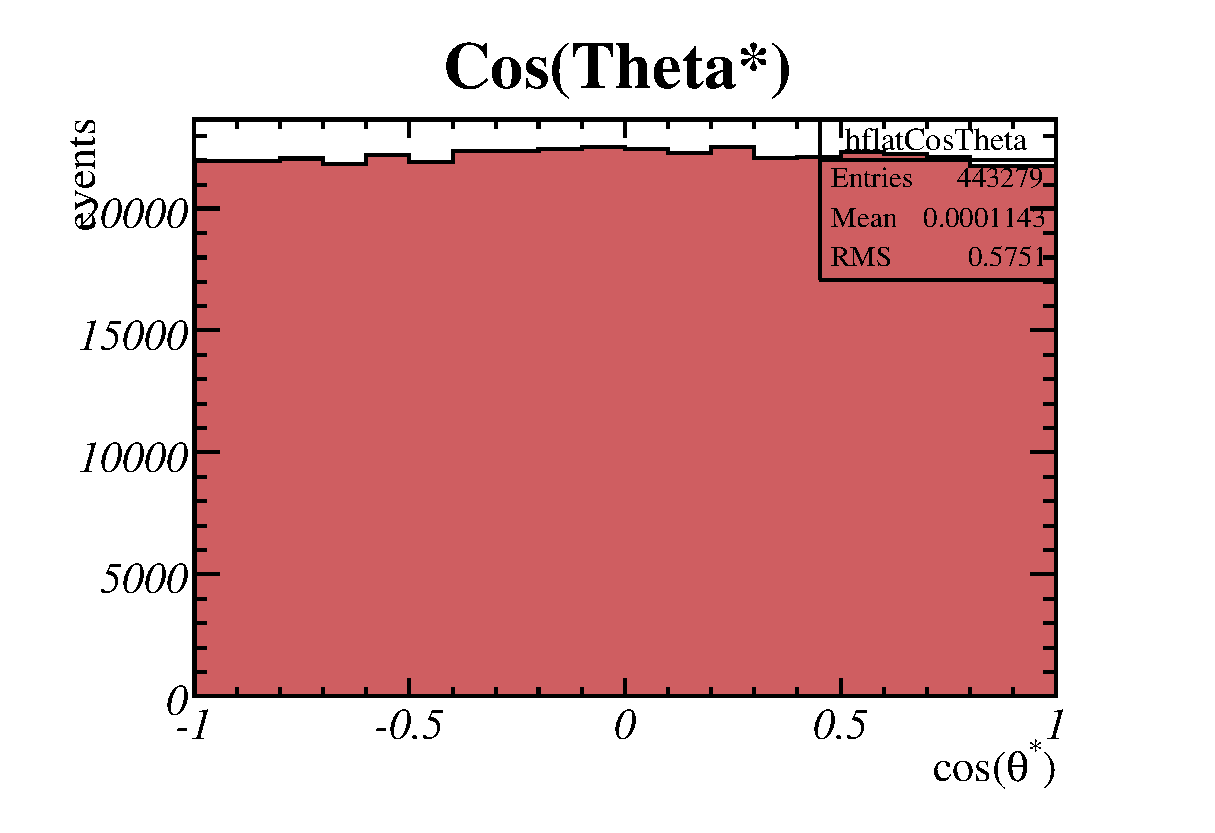
\includegraphics[width=0.48\textwidth]{pics/CosThetaA.eps}}
  \subfigure[]{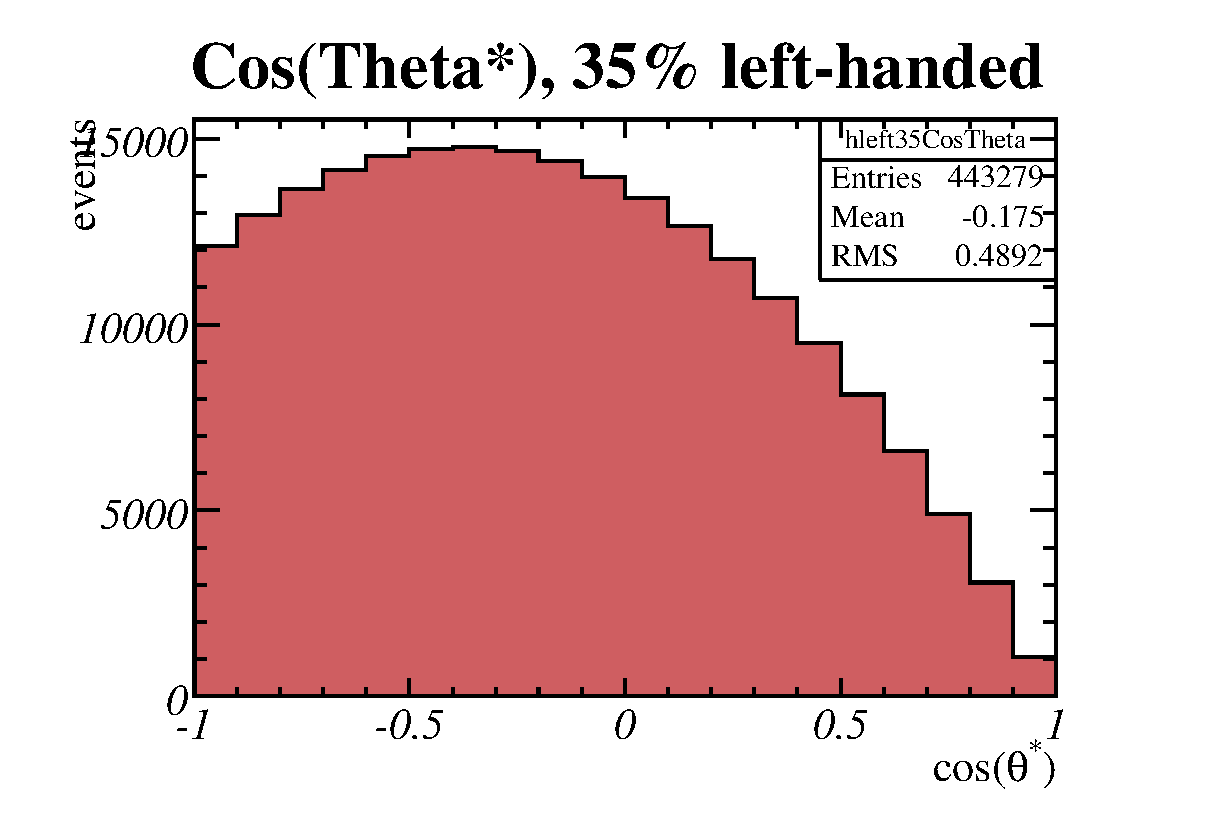
\includegraphics[width=0.48\textwidth]{pics/CosThetaB35left.eps}}
\end{center}
  \caption{Distribution of \costh for the
    FCNC signal MC sample: (a) before re-weighting, (b) after re-weighting
    according to a $Z$ helicity of 65\% longitudinal and 35\%
    left-handed.}
  \label{fig:costheta}
\end{figure}

The helicity of the $W$ from a SM top decay is determined by the fact
that the longitudinal degree of freedom of the $W$ is acquired from the
Higgs field. Any theory beyond the SM must provide a similar mechanism
to create massive gauge bosons; therefore, the best guess for the longitudinal
fraction of the $Z$ helicity, $f^0$, is given by the SM prediction~\cite{Tait}:

\begin{equation}
f^0 = \frac{m_t^{~2}}{2m_Z^{~2} + m_t^{~2}} \approx 0.65.
\end{equation}

The Higgs mechanism does not predict the fraction of left-handed to
right-handed helicity; however, for a $Z$ decay, changing from
left-handed to right-handed is equivalent to looking at the oppositely
charged lepton.  Assuming that the CDF detector is approximately
symmetric with respect to positively and negatively charged leptons,
the acceptance is very similar when switching from a
left-handed to a right-handed decay.

For all acceptance calculations, we re-weight the signal MC sample such
that the $Z$ helicity is 65\% longitudinal and 35\% left/right-handed. Our
ignorance of the exact nature of the interaction is taken into account
by a assigning a corresponding systematic uncertainty, as will be
described in Section~\ref{section:helicitysystematics}.


\subsection{Acceptance}

\subsubsection{Acceptance and Scale Factors}
The acceptance for the FCNC signal MC is determined by applying the
baseline event selection ($Z$ candidate and four jets with $\et>15
\gev$ and $|\eta| <$ 2.4) to the signal MC and then correcting for some known limitations of
the MC simulation. 
%The raw acceptance for our decay channel is 16.79 $\pm$ 0.05\% (stat). 
%When the branching fractions for $Z \rightarrow$ \ee, \mm and \Wqq are taken 
%into account, we get a raw acceptance of 0.76$\pm$0.004\%.

For the $Z$ reconstruction efficiency we have to
take into account the discrepancy between the efficiency to identify a
lepton in data and the MC simulation. These scale factors are not only different for the
different detectors used to identify the leptons, but they also vary among the MC
simulations corresponding to different data taking periods. We apply these scale 
factors on a per-event basis, and take into account the added efficiency from
recovering tight leptons as tracks. Each event receives a scale factor, ${\mathcal SF}$:

\begin{eqnarray*}
{\mathcal SF} & = & \mathcal{SF}_{L1} \cdot \mathcal{SF}_{L2} 
               +  (1-\mathcal{SF}_{L1}) \cdot \mathcal{SF}_{L2} \cdot \mathcal{SF}_{T1} 
               +  (1-\mathcal{SF}_{L2}) \cdot \mathcal{SF}_{L1} \cdot \mathcal{SF}_{T2}. \\
\end{eqnarray*}

In the above equation, ${\mathcal SF}_{L1}$ and ${\mathcal SF}_{L2}$ are the scale factors
for the leptons, and ${\mathcal SF}_{T1}$ and ${\mathcal SF}_{T2}$ are the track scale factors
for the tracks matched these leptons. The added efficiency from recovering both tight 
leptons as tracks appears in the last two terms of the above equation. Note that for 
the case where neither lepton has been matched to a track, both $\mathcal{SF}_{T1}$ 
and $\mathcal{SF}_{T2}$ are zero, and the above equation reduces to the more familiar 
event scale factor for a $Z$ formed from two tight leptons:

\begin{eqnarray*}
{\mathcal SF} & = & \mathcal{SF}_{L1} \cdot \mathcal{SF}_{L2}. \\
\end{eqnarray*}

It is possible to apply the same treatment for the lepton and track trigger efficiencies. 
We ignore the trigger efficiency gain from recovering tight leptons as tracks. Instead, we
assume that all tight leptons fire the trigger, and that phoenix electrons and tracks
would not have. Per event, we assign a weight for the trigger efficiency, 
${\mathcal E}$:

\begin{eqnarray*}
{\mathcal E} & = & \mathcal{E}_{L1} + \mathcal{E}_{L2} 
                        -  \mathcal{E}_{L1} \cdot \mathcal{E}_{L2}. \\
\end{eqnarray*}

In the above efficiency equation, ${\mathcal E}_{L1}$ and ${\mathcal E}_{L2}$ are the trigger 
efficiencies for leptons. The lepton ID scale factors and lepton 
trigger efficiencies are given in Table~\ref{table:sf}. The corrected acceptances for our 
signal Monte Carlo samples are given in Table~\ref{table:acc_cor}.

%Since these scale factors are
%different for the different detectors we use to identify leptons, we
%divide our $Z$ sample by the lepton type of the two legs, CEM, PHX,
%CMUP, CMX (arches or miniskirt/keystone), and track lepton. Then we apply the relevant 
%scale factors to each category. In addition, we apply correction factors for the 
%lepton trigger efficiencies for each lepton type. We only allow tight central electrons and 
%tight muons to trigger. 

%The scale factors for the different detectors are
%given in Table~\ref{table:sf}. In addition there are slight
%differences between the trigger simulation in the MC and the data,
%taken into account via the trigger efficiencies for tight central
%electrons and muons, see Table~\ref{table:e_eff} and
%Table~\ref{table:mu_eff}.
%The raw and
%corrected $Z$ reconstruction efficiencies for the different $Z$ types
%is given in Table~\ref{table:raweff}. 
%Our overall acceptance for the base selection criteria is
%$\mathcal{A}(\ttbar\to Zc\,Wb) = ??$.

\begin{table}[t]
\begin{center}
\caption{\label{table:acc_cor} The corrected acceptances for the FCNC signal Monte Carlo samples in \%,
  shown with statistical uncertainties only.}
\vspace{2mm}
\small\begin{tabular}{c D{;}{\pm}{-1} D{;}{\pm}{-1} D{;}{\pm}{-1} D{;}{\pm}{-1}} 
\toprule
\multicolumn{1}{c}{\bf MC Sample Name }
& \multicolumn{1}{c}{\bf Acceptance } 
& \multicolumn{1}{c}{\bf BR(Z) } 
& \multicolumn{1}{c}{\bf BR(W/Z) } 
& \multicolumn{1}{c}{\bf Acc$\times$BR}\\ 
\midrule
$Z(ll)W(q\overline{q}')$   & 15.95;0.05 & 6.73;0.01 & 67.60;0.27 & 0.73;0.00 \\
$Z(ll)W(l\nu)$             & 2.50;0.05  & 6.73;0.01 & 32.40;0.27 & 0.05;0.00 \\
$Z(ll,\qqbar)Z(ll,\qqbar)$ & 14.76;0.45 & 6.73;0.01 & 69.91;0.06 & 1.39;0.04  \\
\bottomrule
\end{tabular}
\end{center}
\end{table}

\subsubsection{Branching Fractions}
In the FCNC signal MC simulation, we generate \ttbar 
events with one top decaying via the FCNC mode and the other via the \sm 
mode. Ultimately, we are interested in setting a limit on ${\mathcal B}(\tZq)$. 
We have to properly translate the acceptances for \ttbar $\rightarrow 
Zc Wb$ and \ttbar $\rightarrow Zc Zc$ to extract the limit for \tZq. In order to do this, 
we assume ${\mathcal B}(t \rightarrow Wb) + {\mathcal B}(t \rightarrow Zc) = 1$. The different 
decay modes for the \ttbar pair are as follows:
%\begin{center}

\begin{displaymath}
\begin{array}{|r|cc|}
\hline
                                & {\mathcal B}(t \rightarrow Wb) &
{\mathcal B}(t \rightarrow Zc) \\
\hline
{\mathcal B}(t \rightarrow Wb) & {\color[rgb]{0, 0.5, 0}\bw \cdot \bw} &
{\color[rgb]{0, 0, 0.5}\bw \cdot \bz} \\
{\mathcal B}(t \rightarrow Zc) & {\color[rgb]{0, 0, 0.5}\bw \cdot \bz} &
{\color[rgb]{0.5, 0, 0}\bz \cdot \bz} \\
\hline
\end{array}
\end{displaymath}
%\\ \vspace*{-.1in}

where

%\\ \vspace*{-.3in}
\begin{eqnarray*}
\bz & \equiv & {\mathcal B}(t \rightarrow Zc) \textrm{,} \\
\bw & \equiv & {\mathcal B}(t \rightarrow Wb) = 1 - \bz  \textrm{, and} \\
{\color[rgb]{0, 0.5, 0}\bw \cdot \bw} & \textrm{is} & \textrm{the SM \ttbar background.}
\end{eqnarray*}
%\\ \vspace*{-.0in}
%\end{center}

From this, we can derive the number of events we expect, namely,

%\begin{center}
%\vspace*{-.25in}
\begin{eqnarray*}
{\mathcal N}_\textrm{signal} &=& \left( {\color[rgb]{0, 0, 0.5}2 \bz (1
- \bz)} \cdot {\mathcal A}_{WZ} + {\color[rgb]{0.5, 0, 0}\bz^2} \cdot
{\mathcal A}_{ZZ} \right) \cdot \sigma_{t \bar{t}} \cdot \int {\mathcal
L} dt\\
&=& \bz
           \underbrace{ \left( {\color[rgb]{0, 0, 0.5}2 (1 - \bz)} +
{\color[rgb]{0.5, 0, 0}K_{ZZ/WZ} \cdot \bz} \right)}_\textrm{Acceptance
Correction Factor} \cdot
           \overbrace{{\mathcal A}_{WZ}}^\textrm{From MC}  \cdot
\sigma_{t \bar{t}} \cdot \int {\mathcal L} dt,\\
\end{eqnarray*}
%\\ \vspace*{-.1in}

where

%\\ \vspace*{-.3in}
\begin{eqnarray*}
{\mathcal A}_{WZ} & \equiv & \textrm{Acceptance } \cdot \textrm{
efficiency for } t \bar{t} \rightarrow WbZc \textrm{, and} \\
{\mathcal A}_{ZZ} & \equiv & \textrm{Acceptance } \cdot \textrm{
efficiency for } t \bar{t} \rightarrow ZcZc \textrm{, and} \\
K_{ZZ/WZ} & \equiv & \textrm {Ratio of } {\mathcal A}_{ZZ} \textrm{ to }
{\mathcal A}_{WZ} \sim 2 \textrm{ (from MC)}.\\
\end{eqnarray*}

%\end{center}
As shown in the following algebraic expressions, we normalize
to the measured lepton+jets top cross section. Note that the lepton+jets
SECVTX cross section top cross section measurement assumes that the 
top quark can only decay as expected by the SM, \tWb. Consequently, 
we have adjust the lepton+jets top cross section for acceptance 
changes due to possible FCNC top decays. In the algebra that follows, we
show that including the FCNC decay mode to the lepton+jets top
cross section yields an acceptance correction expression that 
is based on the limit we set for the FCNC decay. 
We say that this acceptance correction ``runs'' with the \tZq limit.

We also account for the FCNC signal falling within the SM top cross section
acceptance. We use the top cross section event selection to measure the 
acceptance both in a special FCNC signal MC sample with inclusive decays of 
the $W$ and $Z$, $Z(incl.)W(incl.)$, and in the double FCNC MC sample,
$Z(ll,\qqbar)Z(ll,\qqbar)$.


%Like the previous measurement, we are normalizing to the measured
%lepton+jets SECVTX top cross section. The top cross section
%measurement assumes that the top quark decays only to
%$Wb$. 

%Consequently, we have adjust the top cross section based on the
%limit we set for the FCNC decay. We also account for the FCNC signal
%falling within the top cross section acceptance by measuring the
%acceptance with the top cross section event selection on the Monte
%Carlo sample where one top decays to $Zc$ and the other to $Wb$, where
%we allow all decays of the $Z$ and $W$ bosons and the Monte Carlo
%sample where both tops decay to $Zc$.
  
The formula for the top cross section measurement is given by

\begin{displaymath}
{\tt}_\textrm{``Lepton + Jets''} =
  \frac {{\mathcal N}_{LJ} - B_{LJ}}{{\mathcal A}_{LJ} \cdot \lum},
\end{displaymath}
where \alj{~} is acceptance convoluted with efficiency.
We modify the acceptance to allow for the FCNC decay.

\begin{eqnarray*}
\alj{~}&=& (1-\betaz)^2\cdot\alj{ww} + 2\cdot\betaz(1-\betaz)\cdot\alj{wz}
+ \betaz^2\cdot\alj{zz}\\
&=& \alj{ww} \cdot \left[(1-\betaz)^2 + 2\cdot\betaz(1-\betaz)\cdot\rlj{wz}
+ \betaz^2\cdot\rlj{zz}\right]\\
\end{eqnarray*}
%\\ \vspace*{-.25in}

where

%\\ \vspace*{-.2in}
\begin{eqnarray*}
\rlj{wz}&\equiv&\frac{\alj{wz}}{\alj{ww}}\\
\rlj{zz}&\equiv&\frac{\alj{zz}}{\alj{ww}}\\
\end{eqnarray*}
%\\ \vspace*{-.3in}
This gives an enhancement to the top cross section as shown below.

\begin{eqnarray*}
{\tt}_\textrm{``Lepton + Jets''}
  & = &   \frac {{\mathcal N}_{LJ} - B_{LJ}}
{{\mathcal A}_{LJ} \cdot \lum} \\
  & = & \overbrace{\frac{1}
{(1-\betaz)^2 + 2\cdot\betaz(1-\betaz)\cdot\rlj{wz} + \betaz^2 \cdot
\rlj{zz}}}^
\textrm{Enhancement Factor}\\
& &{\bf \cdot} \underbrace{\frac {{\mathcal N}_{LJ} - B_{LJ}}
{\alj{ww} \cdot \lum}}_\textrm{Standard Cross Section} \\
\end{eqnarray*}
Inserting this top cross section back into our calculation for the
number of events gives

\label{eq:fullacc}
\begin{eqnarray*}
{\mathcal N}_\textrm{signal} &=& \bz
           \left( 2 (1 - \bz) + K_{ZZ/WZ} \cdot \bz \right) \cdot
           {\mathcal A}_{WZ} \cdot \\
& & \sigma_{t \bar{t}} \cdot \int {\mathcal L} dt\\
&=&  \bz
           \left( 2 (1 - \bz) + K_{ZZ/WZ} \cdot \bz \right) \cdot
           {\mathcal A}_{WZ} \cdot \\
& & 
  \frac{1}
{(1-\betaz)^2 + 2\cdot\betaz(1-\betaz)\cdot\rlj{wz} + \betaz^2 \cdot
\rlj{zz}}
{\bf \cdot} \frac {{\mathcal N}_{LJ} - B_{LJ}}
{\alj{ww} \cdot {\color[rgb]{0, 0.5, 0} \lum}} \cdot {\color[rgb]{0,
0.5, 0}\lum} \\
&=&  \bz {\bf \cdot}
  ( {\mathcal N}_{LJ} - B_{LJ}) \cdot {\color[rgb]{0, 0, 0.5} \frac {
{\mathcal A}_{WZ} } {\alj{ww}}}
\cdot
{\color[rgb]{0.5, 0, 0}
\underbrace{ \frac{\left( 2 \cdot (1 - \bz) + K_{ZZ/WZ} \cdot \bz \right)}
{(1-\betaz)^2 + 2\cdot\betaz(1-\betaz)\cdot\rlj{wz} + \betaz^2 \cdot
\rlj{zz}}
}_\textrm{Full Running Acceptance Correction} }
  \\
\end{eqnarray*}

Both the lepton+jets acceptances \alj{ww}, \alj{wz},
and \alj{zz} and the FCNC acceptances ${\mathcal A}_{WZ}$ and ${\mathcal A}_{ZZ}$
in the above calculation are measured in the Monte Carlo simulation. Additionally, the 
normalization to the measured top cross section removes our
dependence on luminosity uncertainties. Using the ratio of acceptances, 
many of our systematic uncertainties also partially cancel; however, we 
assign a systematic uncertainty for the statistical and systematic 
uncertainties on the number of lepton+jets candidates and background estimate.
 
%There is an extra factor of
%two since either top may decay via the FCNC mode. 
%The number of
%expected signal events given the branching fraction of the FCNC decay
%$\br(\tZc)$ to be measured, the \ttbar \xsect $\sigma_\ttbar$, and the
%integrated luminosity \Lint is then given by
%\begin{eqnarray}
%N_{\ttbar\to Zc\,Wb}&=& 2\cdot \br(\tZc) \cdot \left\{1-\br(\tZc)\right\} \cdot\\ \nonumber
%&&\left\{\br(\Zee) + \br(\Zmm)\right\}\cdot\br(\Wqq) \cdot\\ \nonumber
%&&\mathcal{A}(\ttbar\to Zc\,Wb)\cdot\sigma_\ttbar \cdot \Lint.
%\end{eqnarray}
%Additional acceptance is gained from the double FCNC decay $\ttbar \to
%Zc\,Zc$. In this case the MC simulation allows both $Z$s to
%independently decay into \ee, \mm, or \qqbar, and the number of expected events is
%\begin{eqnarray}
%N_{\ttbar\to Zc\,Zc}&=& \br(\tZc)^2 \cdot\\ \nonumber
%&& \left\{\br(\Zee) + \br(\Zmm) + \br(\Zqq)\right\}^2 \cdot\\ \nonumber
%&&\mathcal{A}(\ttbar\to Zc\,Zc)\cdot\sigma_\ttbar \cdot \Lint.
%\end{eqnarray}

%Our acceptance for the base selection criteria is composed of, in
%addition to the geometric acceptance, the Z reconstruction efficiency
%and the efficiency to find four or more jets. 
%For our optimized selection criteria, there are extra efficiencies from the extra selection requirements. Table \# gives the efficiencies for the jet 
%E$_T$, Mass $\chi^2$, transverse mass M$_T$, and H$_T$. The overall acceptance for the optimized selection criteria is x.xx\%. 

\subsection{Tagging Efficiency}
\label{section:tageff}
Simply taking the fraction of $b$-tagged events in the MC simulation
as the tagging efficiency is insufficient due to the fact that the
tagging efficiency in data is lower than in the MC simulation for
heavy flavor jets and the mistag rate, \ie the fraction of
light flavor jets that are falsely tagged, is higher in data than in
the MC simulation. We correct for these discrepancies in the data and
MC tag rates on a jet-by-jet basis.

We identify heavy flavor jets in the MC simulation by matching $b$ and
$c$ hadrons from the list of observed particles (OBSP) to jets in the
event. If a $b$ or $c$ hadron is within an $(\eta,\phi)$ cone of
$\Delta R<0.4$ of a jet, we consider that jet to be a heavy flavor
jet, otherwise a jet is classified as a light flavor jet. In addition, 
heavy flavor jets that are not $b$-tagged in the MC are considered
untagged. We re-weight the number of tagged heavy flavor jets by the 
$b$-tagging scale factor, as shown in Table~\ref{table:tagging_sf}.

For light flavor jets we ignore the tagging information from the
MC simulation.  Instead we get an estimate for the background from
mistagged light flavor jets by applying the Gen6 mistag
parameterization~\cite{CDF7326,CDF8519}. The mistag parameterization contains the
probability for a light jets to be tagged as a function of the jet
kinematics $(\et, |\eta|)$, and event properties (number of tracks per tag,
\et, $|\eta|$, the number of tags, the number of $Z$ vertices, and the 
$v_{z}$ of the primary vertex). The entries of the mistag matrix are determined
from negative tags in generic dijet data.  The mistag parameterization includes
the $\alpha\beta$ correction~\cite{CDF7585,CDF8626}, which accounts for
asymmetries in the positive and the negative tag rates due to decays
of long-lived $K^0_S$ and $\Lambda$ particles, photon conversions, and
material interactions. 

To account for all these corrections, we assign a weight to each MC
event that represents the probability that at least one of the jets in
the event is tagged, either as a genuine heavy flavor jet or as a
mistagged light flavor jet:

\begin{eqnarray}
P_{\text{event,tag}}
&=& 1 - \prod_i\, \text{probability that jet $i$ is not tagged}\\\nonumber
&=& 1 - 
\prod_j \left( 1 - P_{\mathrm{mistag, j}}\right) \cdot
\prod_k \left( 1 - \mathcal{SF}_k \right) \cdot
\prod_l 1.
\end{eqnarray}

Here the index $i$ runs over all jets, $j$ runs over all light flavor
jets, $k$ runs over all tagged and matched heavy flavor jets, and $l$
runs over the remaining non-tagged but matched heavy flavor
jets. ${P}_\mathrm{mistag, j}$ is the mistag probability, and 
$\mathcal{SF}_k$ is the tagging scale factor. The final event tagging 
efficiency of a given MC sample is then given by the sum of all 
per-event weights divided by the number of events.

For signal events satisfying our base selection criteria, the event
tagging efficiencies and, consequently, the efficiencies for the 
signal events to be anti-tagged are given in Table~\ref{table:tag_eff}, 
for the different signal Monte Carlo samples.

We want to set a limit for \tZq while our main signal Monte Carlo samples 
are \tZc. Since the tagging rate for $c$ and $u$ are different, we check 
for the effect of having $Zc$ versus $Zu$ on the tagging efficiency for the 
signal. We check the loose \btag rates in the \ttbar $\rightarrow Zu Wb$ sample and find that 
the tagging efficiency for this sample is $91\pm1\%$ of the tagging efficiency for 
the \ttbar $\rightarrow Zc Wb$ sample. More information on the effect of this
assigned efficiency can be found in Section~\ref{section:systematics}.
%For events satisfying our optimized selection criteria, the event tagging
%efficiency is xx.xx\% and the event anti-tagging efficiency is
%xx.xx\%.

\begin{table}[t]
\begin{center}
\caption{\label{table:tagging_sf} The scale factors used to scale
  the $b$-tagging efficiency of the SECVTX algorithm in the MC
  simulation~\cite{BTagging}.}
\vspace{2mm} 
\small\begin{tabular}{l D{;}{\pm}{-1} D{;}{\pm}{-1}D{;}{\pm}{-1}} \toprule
{\bf Tagger} & \multicolumn{1}{c}{\bf Scale Factor} \\
\midrule
Loose SECVTX & 0.95;0.05\\
Tight SECVTX & 0.95;0.04\\
\bottomrule
\end{tabular}
\end{center}
\end{table}

\begin{table}[t]
\begin{center}
\caption{\label{table:tag_eff} Loose SECVTX tagging efficiencies for signal 
  Monte Carlo samples.}
\vspace{2mm} 
\small\begin{tabular}{c D{;}{\pm}{-1} D{;}{\pm}{-1}} \toprule
& \multicolumn{1}{c}{\bf Tag Efficiency } 
& \multicolumn{1}{c}{\bf Anti-tag Efficiency}\\ 
\midrule
$Z(ll)W(q\overline{q}')$  & 54.6;0.2\% & 45.4;0.1\% \\
$Z(ll)W(l\nu)$            & 51.6;0.6\% & 48.4;0.6\% \\
$Z(ll)uW(q\overline{q}')$ & 37.5;1.4\% & 62.5;2.3\% \\
\bottomrule
\end{tabular}
\end{center}
\end{table}

% CHARLES: probably moved this section to later in the note...
%\subsubsection{Cut Optimization}
%Additional cuts on the transverse momenta of the jets, the transverse
%mass \mt, and the mass $\chi^2$ are applied on top of the base
%selection. The actual values of the cuts are optimized for the
%best expected limit on $\br(\tZq)$. The cut optimization and the
%signal acceptance at the optimal point are discussed in
%Section~\ref{section:optvariables}. After optimization 71\% of the tagged 
%signal and 56\% of the anti-tagged signal remain compared to base cuts.
	
% We again
%throw a random number between zero and one. If the resulting number is
%more than the mistag rate, we count the light flavor jet as
%untagged. If the number is less, we assign the jet as tagged.

% If a heavy flavor jet is tagged, we throw a
%random number between zero and one. If the resulting number is less
%than the scale factor, we keep the tag for the heavy flavor jet. If it
%is higher, we consider the jet untagged. Therefore, all the heavy
%flavor jets as a whole get scaled down by the scale factor.

%After having assigned tags on a jet-by-jet basis according to the
%scale factor and mistag rates, we count the total number of tags in
%each event and take the fraction of events with one or more tags as
%the event tagging efficiency. 

